\documentclass[11pt, spanish, a4paper, twoside]{article}

% Versión 1.er cuat 2021 Víctor Bettachini < vbettachini@unlam.edu.ar >

\usepackage[T1]{fontenc}
\usepackage[utf8]{inputenc}

\usepackage[spanish, es-tabla]{babel}
\def\spanishoptions{argentina} % Was macht dass?
% \usepackage{babelbib}
% \selectbiblanguage{spanish}
% \addto\shorthandsspanish{\spanishdeactivate{~<>}}

\usepackage{graphicx}
\graphicspath{{./figuras/}{../LaTeX/}}
% \usepackage{float}

\usepackage[arrowdel]{physics}
\newcommand{\pvec}[1]{\vec{#1}\mkern2mu\vphantom{#1}}
% \usepackage{units}
\usepackage[separate-uncertainty= true, multi-part-units= single, range-units= single, range-phrase= {~a~}, locale= FR]{siunitx}
\usepackage{isotope} % $\isotope[A][Z]{X}\to\isotope[A-4][Z-2]{Y}+\isotope[4][2]{\alpha}

\usepackage{tasks}
\usepackage[inline]{enumitem}
% \usepackage{enumerate}

\usepackage{hyperref}

% \usepackage{amsmath}
% \usepackage{amstext}
% \usepackage{amssymb}

\usepackage{tikz}
\usepackage{tikz-dimline}
\usetikzlibrary{calc}
% \usetikzlibrary{math}
\usetikzlibrary{arrows.meta}
\usetikzlibrary{snakes}
\usetikzlibrary{decorations}
\usetikzlibrary{decorations.pathmorphing}
\usetikzlibrary{patterns}

\usepackage[hmargin=1cm,vmargin=3cm, top= 0.75cm,nohead]{geometry}

\usepackage{lastpage}
\usepackage{fancyhdr}
\pagestyle{fancyplain}
\fancyhf{}
\setlength\headheight{28.7pt} 
\fancyhead[LE, LO]{\textbf{Mecánica General} }
\fancyhead[RE, RO]{\href{https://ingenieria.unlam.edu.ar/}{$\vcenter{\hbox{
\includegraphics[height=1cm]{ambos.pdf}}}$}}
\fancyfoot{\href{https://creativecommons.org/licenses/by-nc-sa/4.0/deed.es_ES}{$\vcenter{\hbox{
\includegraphics[height=0.4cm]{by-nc-sa_80x15.pdf}}}$} \href{https://ingenieria.unlam.edu.ar/}{DIIT - UNLaM}}
\fancyfoot[C]{ {\tiny Actualizado al \today} }
\fancyfoot[RO, LE]{Pág. \thepage/\pageref{LastPage}}
\renewcommand{\headrulewidth}{0pt}
\renewcommand{\footrulewidth}{0pt}


\begin{document}
\begin{center}
  % \textsc{\large Mecánica general}\\
  \textsc{\large Cuerpo rígido | Tensores de inercia}
\end{center}

% De poder resolver estos problemas en forma autónoma puede asumir que adquirió los conocimientos mínimos sobre los temas abordados en la semana. No dude en consultar a docentes y compañeros si no puede terminarlos.
% Los problemas marcados con (*) son opcionales.

\begin{enumerate}

% \vspace{-.5cm}
% \section*{Tensores de inercia}


\item Se tiene una barra de \(m= \SI{1}{\kilo\gram}\) de sección despreciable frente a \(l= \SI{1}{\metre}\).
De alinear un eje (\(\hat{z}\)) con ella, 
\begin{tasks}(2)
	\task	¿cuales son sus momentos de inercia?,
	\task ¿existen los productos de inercia? 
\end{tasks}


\item
Dibuje sistemas de ejes conveniente para calcular momentos de inercia.
\vspace{-1.1cm}
\begin{tasks}(4)
	\task 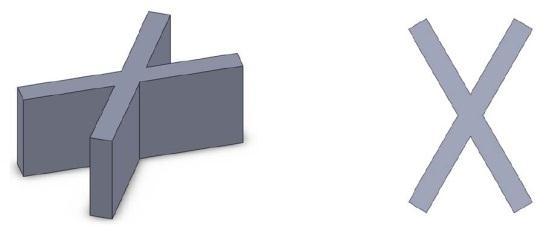
\includegraphics[width=0.15\textwidth]{o-000}
	\task 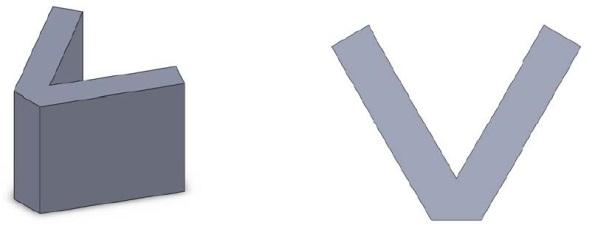
\includegraphics[width=0.15\textwidth]{o-001}
	\task 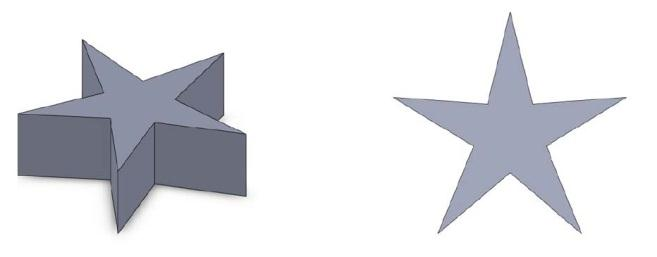
\includegraphics[width=0.15\textwidth]{o-002}
	\task 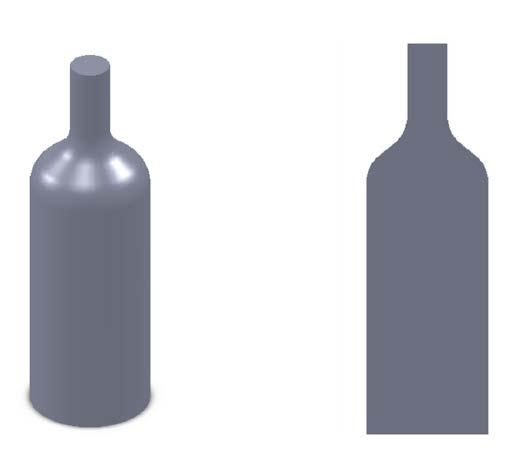
\includegraphics[width=0.15\textwidth]{o-003}
\end{tasks}



\item 
\begin{minipage}[t][4.5cm]{0.7\textwidth}
Calcule para el sistema de ambas $m$ (la masa de brazos y ejes es despreciable)
\begin{tasks} 
	\task tensor de inercia \(\overline{\overline{I}}\) respecto a A,
	\task momento angular $\vec{L}\bigg\rvert_A = \overline{\overline{I}} \vec{\Omega}$ y torque $\vec{\tau} = \dot{\vec{L}}$.
\end{tasks}
La porción vertical de la barra se mantiene con rulemanes que impiden su movimiento vertical, pero posibilitan que el eje rote sin fricción con velocidad angular $\Omega$, que puede no ser constante, respecto el marco inercial $O_{xyz}$.
\end{minipage}
\begin{minipage}[c][0cm][t]{0.25\textwidth}
	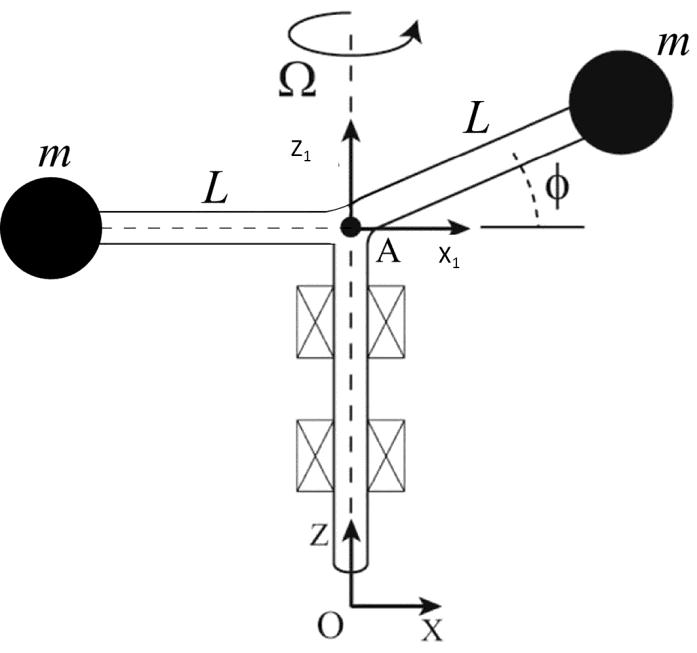
\includegraphics[width=\textwidth]{o-021}
\end{minipage}



\item Calcule los momentos de inercia para una molécula de \isotope{H_2O}.\\
En CNPT se abre con un ángulo de \ang{104,5;;} y median \SI{95.84}{\pico\metre} entre \isotope{O} y \isotope{H}.



\item 
\begin{minipage}[t][3.7cm]{0.6\textwidth}
% \begin{minipage}[t][3.5cm]{0.7\textwidth}
% Tensor de inercia de un cubo con arista \(b\).
\textbf{Marion (e) ex. 11-3} Tensor de inercia de un cubo con arista \(b\).
	\begin{enumerate}
	\item Calcule el tensor de inercia desde el sistema de ejes \(x_i\) con origen en el centro de masa \(O\).
	\item Use la forma general del teorema de ejes paralelos de Steiner para calcularlo en el sistema \(X_i\) con origen en el vértice \(Q\) 
	\end{enumerate}
\end{minipage}
\begin{minipage}[c][1.2cm][t]{0.35\textwidth}
	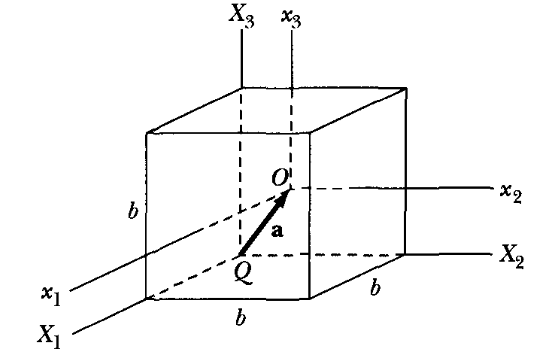
\includegraphics[width=\textwidth]{mFig11-8}
\end{minipage}



\item 
\begin{minipage}[t][3.5cm]{0.5\textwidth}
En una plancha metálica se calaron dos aberturas en forma simétrica.
Esta \emph{penduléa} desde el punto A manteniendose siempre en el plano \(x,y\) por lo que es relevante conocer su momento de inercia \(I_{zz}\).
Por pesado se determinó la $m$ de la planchuela calada y se midieron todas las dimensiones que indica la figura.
Calcule \(I_{zz}\) desde A en función de esos datos.
\end{minipage}
\begin{minipage}[c][1.5cm][t]{0.45\textwidth}
	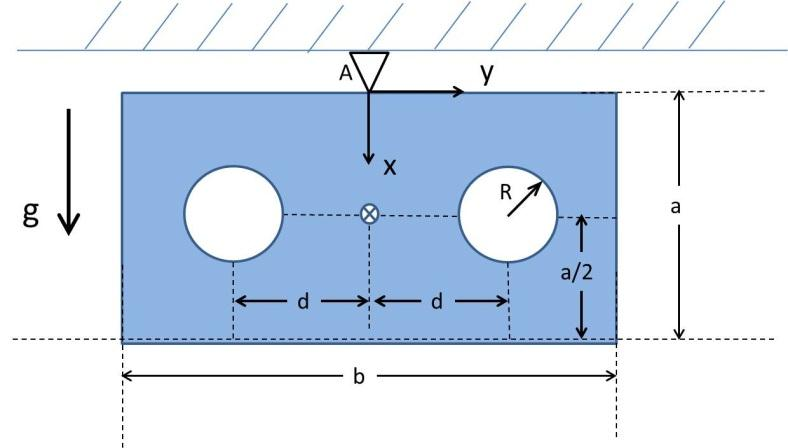
\includegraphics[width=\textwidth]{o-023}
\end{minipage}



\item 
\begin{minipage}[t][1.3cm]{0.65\textwidth}
\textbf{Landau \S 32 6}\\%Hallar la energía cinética de un cilindro homogéneo de radio \(a\) que rueda en el interior de una superficie cilíndrica de radio \(R\).
	Hallar la energía cinética de un cilindro homogéneo de radio \(a\) que rueda en el interior de una superficie cilíndrica de radio \(R\).
\end{minipage}
\begin{minipage}[c][1.5cm][t]{0.3\textwidth}
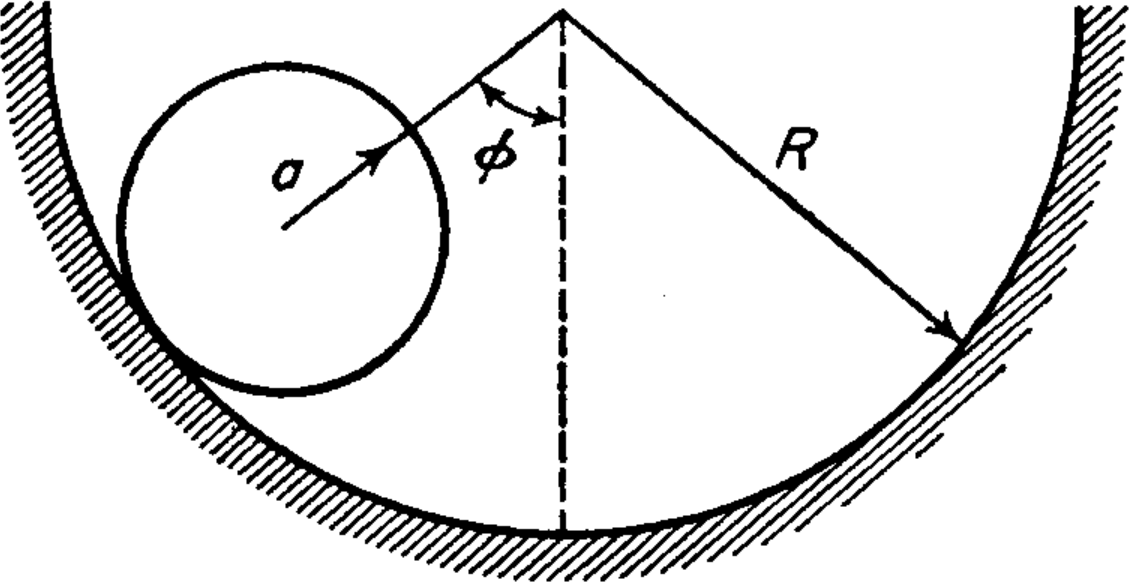
\includegraphics[width=\textwidth]{lFig41}
\end{minipage}



\item 
\begin{minipage}[t][3.5cm]{0.5\textwidth}
\textbf{Landau \S 32 2e} y \textbf{Landau \S 32 7}\\
Calcule:
	\begin{enumerate}
		% \item \textbf{Landau \S 32 2e} Calcule los momentos principales de inercia de un cono homogéneo de altura \(h\) y radio \(R\).
		\item En un sistema de ejes conveniente calcule el tensor de inercia de este cono homogéneo de altura \(h\) y radio en su base \(R\).
		\item Energía cinética de dicho cono rodando sobre el plano \(X Y\).
		El contacto instantáneo \(\overline{O A}\) forma un ángulo de \(\theta\) con \(\hat{X}\).
		% \textbf{Landau \S 32 7} Hallar la energía cinética de un cono homogéneo que rueda sobre un plano.
	\end{enumerate}
\end{minipage}
\begin{minipage}[c][1cm][t]{0.45\textwidth}
	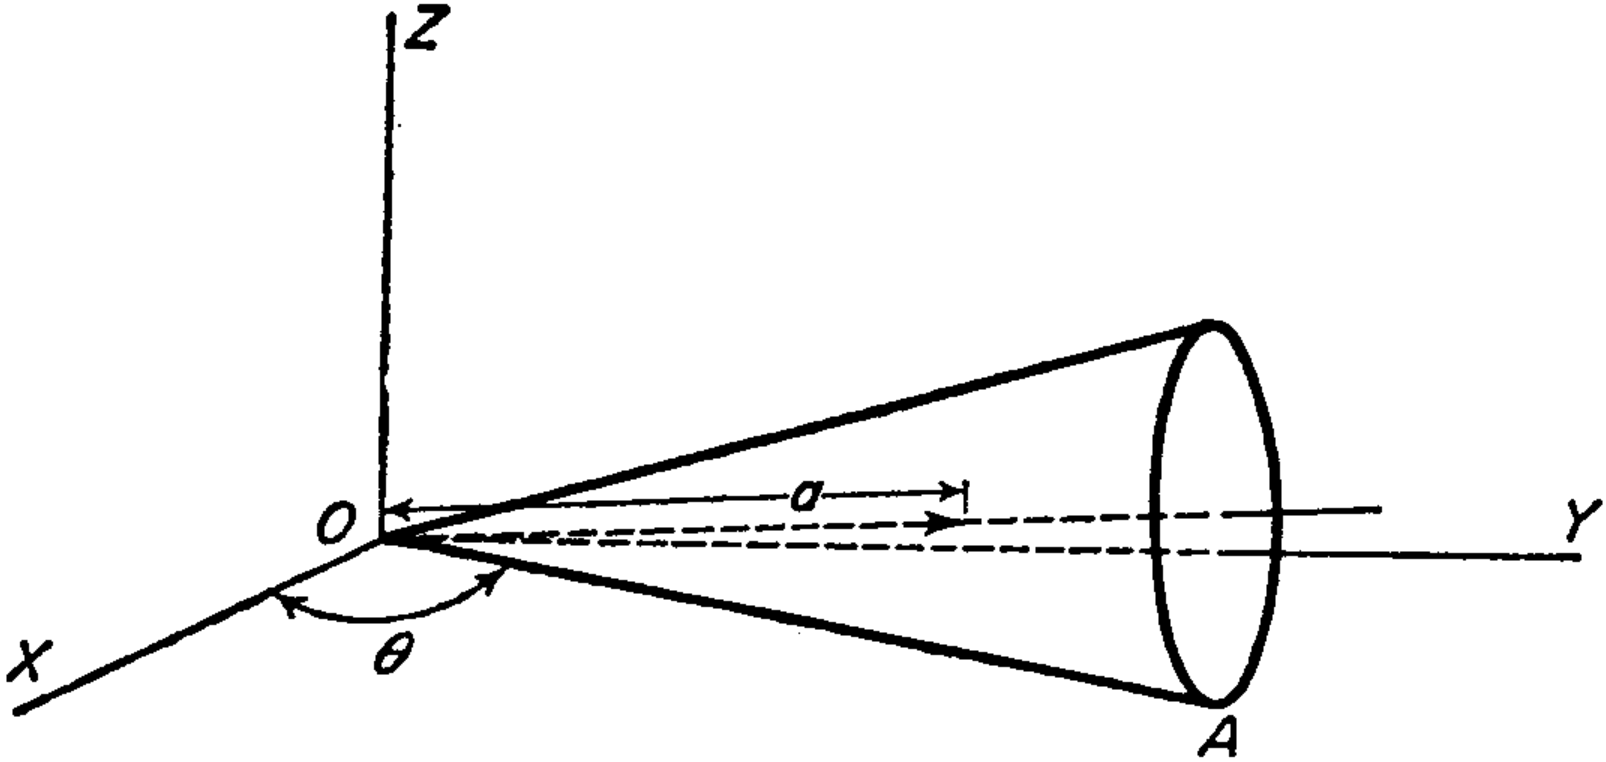
\includegraphics[width=\textwidth]{lFig42}
\end{minipage}




\end{enumerate}
\end{document}
